% Pooling vs Ensembling for Ridge Regression Under Covariate Shift
% 30-slide talk + backup. Compile with: tectonic slides.tex
\documentclass[aspectratio=169,11pt]{beamer}

\usepackage{amsmath,amssymb,bm}
\usepackage{graphicx}
\usepackage{tikz}
\usetikzlibrary{arrows.meta,positioning,calc}

% ---------- theme ----------
\usetheme{default}
\usecolortheme{seahorse}
\definecolor{navy}{RGB}{18,54,96}
\definecolor{poolblue}{RGB}{31,119,180}
\definecolor{ensorange}{RGB}{230,105,20}
\definecolor{wingreen}{RGB}{34,120,60}
\definecolor{softgray}{RGB}{120,120,120}
\setbeamercolor{structure}{fg=navy}
\setbeamercolor{frametitle}{fg=navy,bg=white}
\setbeamercolor{title}{fg=navy}
\setbeamerfont{frametitle}{series=\bfseries,size=\large}
\setbeamertemplate{navigation symbols}{}
\setbeamertemplate{footline}{%
  \hfill\textcolor{softgray}{\scriptsize\insertframenumber\,/\,\inserttotalframenumber}\hspace{2mm}\vspace{2mm}}
\setbeamertemplate{itemize item}{\textcolor{navy}{$\blacktriangleright$}}
\setbeamertemplate{itemize subitem}{\textcolor{softgray}{--}}

\newcommand{\takeaway}[1]{%
  \vfill
  {\centering\colorbox{navy!8}{\parbox{0.92\textwidth}{\centering\small\textcolor{navy}{#1}}}\par}}

\newcommand{\E}{\mathbb{E}}
\newcommand{\R}{\mathbb{R}}
\newcommand{\Tr}{\operatorname{Tr}}
\newcommand{\bbeta}{\bm{\beta}}
\newcommand{\bmu}{\bm{\mu}}
\newcommand{\X}{\mathbb{X}}

\title{\LARGE Pooling Versus Ensembling for Ridge Regression\\ Under Covariate Shift}
\author{Maya Ramchandran}  % TODO: add coauthors
\institute{NeurIPS 2026 submission}
\date{}

\begin{document}

% ---------- 1 ----------
\begin{frame}
  \titlepage
\end{frame}

% ---------- 2 ----------
\begin{frame}{Motivation}
  \begin{itemize}
    \item Datasets often partition naturally into clusters: sub-populations, batch effects, multiple studies or sources
    \item Two standard strategies for prediction: fit a single model to the pooled data, or fit one model per cluster and combine the predictions
  \end{itemize}
  \vspace{1mm}
  \begin{center}
  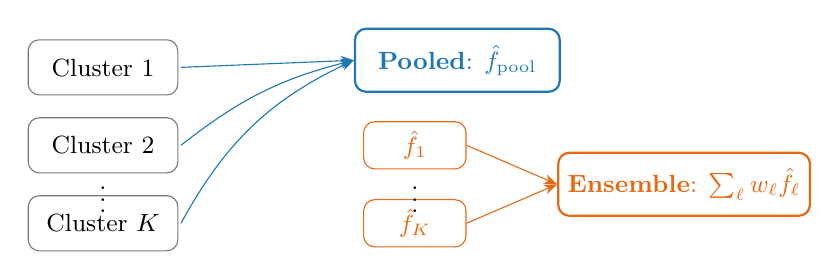
\begin{tikzpicture}[scale=0.9, every node/.style={font=\small}]
    % clusters
    \foreach \y/\lab in {0/{Cluster 1}, -1.1/{Cluster 2}, -2.2/{Cluster $K$}}{
      \node[draw=softgray, rounded corners, minimum width=1.9cm, minimum height=0.7cm] (c\lab) at (0,\y) {\lab};
    }
    \node at (0,-1.75) {$\vdots$};
    % pooled path
    \node[draw=poolblue, thick, rounded corners, minimum width=2.6cm, minimum height=0.8cm, text=poolblue] (pool) at (5,0.1) {\textbf{Pooled}: $\hat f_{\mathrm{pool}}$};
    % ensemble path
    \foreach \y/\l in {-1.1/1, -2.2/K}{
      \node[draw=ensorange, rounded corners, minimum width=1.3cm, minimum height=0.55cm, text=ensorange] (m\l) at (4.4,\y) {$\hat f_{\l}$};
    }
    \node at (4.4,-1.75) {$\vdots$};
    \node[draw=ensorange, thick, rounded corners, minimum width=2.7cm, minimum height=0.8cm, text=ensorange] (ens) at (8.2,-1.65) {\textbf{Ensemble}: $\sum_\ell w_\ell \hat f_\ell$};
    \draw[-{Stealth}, poolblue] (1.1,0) -- (pool.west);
    \draw[-{Stealth}, poolblue] (1.1,-1.1) to[bend left=12] (pool.west);
    \draw[-{Stealth}, poolblue] (1.1,-2.2) to[bend left=18] (pool.west);
    \draw[-{Stealth}, ensorange] (m1.east) -- (ens.west);
    \draw[-{Stealth}, ensorange] (mK.east) -- (ens.west);
  \end{tikzpicture}
  \end{center}
  \vspace{1mm}
  There is limited theoretical guidance on when the second strategy is preferable.
\end{frame}

% ---------- 3 ----------
\begin{frame}{Empirical background}
  \begin{itemize}
    \item In multi-study settings, ensembles of study-specific learners have repeatedly been observed to generalize more reliably than models trained on merged data
    \item This has been documented for a range of base learners, including neural networks, random forests, and regularized regression
    \item Cross-study weighting schemes for such ensembles have been developed in this line of work
  \end{itemize}
  \vspace{2mm}
  {\small\textcolor{softgray}{Patil \& Parmigiani (2018); Guan et al.\ (2019); Ramchandran et al.\ (2020); Trivedi et al.\ (2015)}}
\end{frame}

% ---------- 4 ----------
\begin{frame}{Two closely related lines of work}
  \begin{block}{\small Ramchandran \& Mukherjee (2021)}
    \small Studied the same setting as ours --- covariate shift with no concept shift --- for \textbf{random forests}, and found that ensembling performs well. This motivates a closer look at whether the same holds for linear methods.
  \end{block}
  \vspace{1mm}
  \begin{block}{\small Patil et al.\ (2023)}
    \small Exact risk characterization for subsampling ensembles (subagging, splagging) of ridge and ridgeless learners, under i.i.d.\ data and uniformly random partitions. They show that properly tuned ridge is optimal among the methods considered.
  \end{block}
  \vspace{2mm}
  \textbf{This work:} extend the exact-risk analysis to heterogeneous clusters, with the partition following the true cluster structure, using ridge regression as the base learner.
\end{frame}

% ---------- 5 ----------
\begin{frame}{Question and main results}
  \begin{block}{}
    \centering When the outcome model is shared across clusters, does cluster-aware ensembling\\ offer any advantage over pooling for ridge regression?
  \end{block}
  \vspace{3mm}
  Setting: ridge-regularized least squares, shared $\bbeta$, cluster-specific covariate means, proportional asymptotics $p/n \to \gamma$.
  \vspace{2mm}
  \begin{itemize}
    \item<2-> For any optimally tuned $\lambda > 0$, the \textcolor{poolblue}{\textbf{pooled predictor outperforms the ensemble}}, uniformly over cluster configurations
    \item<2-> For the ridgeless predictor ($\lambda = 0$), the ensemble is preferable only in a specific regime between the two interpolation thresholds
    \item<2-> The mechanism behind that exception is implicit regularization, not cluster structure
  \end{itemize}
\end{frame}

% ---------- 6 ----------
\begin{frame}{Setup}
  \begin{columns}[T]
    \column{0.55\textwidth}
    \begin{itemize}
      \item $K$ clusters; within cluster $\ell$, covariates have mean $\bmu_\ell$ and shared covariance $\Sigma$
      \item The coefficient vector $\bbeta$ is the same in every cluster and at test time
      \item Test point: centered, isotropic
    \end{itemize}
    \vspace{2mm}
    {\small\textcolor{softgray}{Mean shifts keep the analysis tractable while capturing a central form of between-cluster variation (Remark 2.2); cluster labels are treated as known.}}
    \column{0.42\textwidth}
    \begin{align*}
      \bm{X}_{i,\ell} &= \bmu_\ell + \Sigma^{1/2}\bm{Z}_{i,\ell}\\[1mm]
      Y_{i,\ell} &= \bbeta^\top \bm{X}_{i,\ell} + \varepsilon_{i,\ell}\\[1mm]
      p/n_\ell &\to \gamma_\ell \in [0,\infty)
    \end{align*}
  \end{columns}
  \takeaway{Clusters differ only through their covariate distributions; the regression function is shared.}
\end{frame}

% ---------- 7 ----------
\begin{frame}{The two estimators}
  \textbf{Pooled} ridge on all $n = \sum_\ell n_\ell$ samples:\qquad
  $\hat\bbeta_{\lambda_0} = (\X_{\mathrm{pool}}^\top \X_{\mathrm{pool}} + \lambda_0 \mathbb{I})^{-1}\X_{\mathrm{pool}}^\top \bm{Y}_{\mathrm{pool}}$
  \vspace{2mm}

  \textbf{Ensemble}: per-cluster ridge, convex weights:\qquad
  $\hat\bbeta_{\mathrm{ens}}(\bm w) = \sum_{\ell=1}^{K} w_\ell\, \hat\bbeta_{\lambda_\ell}, \quad w_\ell \ge 0,\ \textstyle\sum_\ell w_\ell = 1$
  \vspace{2mm}

  \textbf{Ridgeless} ($\lambda \downarrow 0$): minimum-norm least squares via the pseudoinverse
  \vspace{3mm}
  \begin{itemize}
    \item Same base learner and same data; only the combination strategy differs
    \item Both methods are given optimal tuning parameters and, for the ensemble, optimal weights
  \end{itemize}
\end{frame}

% ---------- 8 ----------
\begin{frame}{The aspect ratio and double descent}
  \begin{columns}[T]
    \column{0.46\textwidth}
    \vspace{2mm}
    \begin{itemize}
      \item The pooled learner has aspect ratio $\gamma_0 = p/n$; each base learner has $\gamma_\ell = p/n_\ell \approx K\gamma_0$
      \item Splitting the data increases the effective aspect ratio by a factor of $K$
      \item Ridgeless risk diverges at $\gamma = 1$ and decreases beyond it (Hastie et al., 2022); ridge regularization removes the peak
    \end{itemize}
    \column{0.52\textwidth}
    \begin{center}
    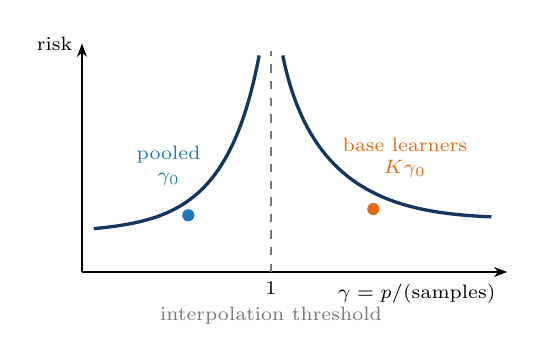
\begin{tikzpicture}[scale=1.0, every node/.style={font=\scriptsize}]
      \draw[-{Stealth}] (0,0) -- (5.4,0) node[below left=1pt] {$\gamma = p/\text{(samples)}$};
      \draw[-{Stealth}] (0,0) -- (0,2.9) node[left] {risk};
      \draw[very thick, navy]
        (0.15,0.55) .. controls (1.2,0.65) and (1.9,0.9) .. (2.25,2.75);
      \draw[very thick, navy]
        (2.55,2.75) .. controls (2.9,1.0) and (4.0,0.75) .. (5.2,0.7);
      \draw[dashed, softgray] (2.4,0) node[below, black] {$1$} -- (2.4,2.8);
      % positions
      \fill[poolblue] (1.35,0.72) circle (2.2pt);
      \node[poolblue, align=center] at (1.1,1.35) {pooled\\ $\gamma_0$};
      \fill[ensorange] (3.7,0.8) circle (2.2pt);
      \node[ensorange, align=center] at (4.1,1.45) {base learners\\ $K\gamma_0$};
      \node[softgray] at (2.4,-0.55) {interpolation threshold};
    \end{tikzpicture}
    \end{center}
  \end{columns}
  \takeaway{Ensembling does not change the base learner; it changes where each learner sits relative to the interpolation threshold.}
\end{frame}

% ---------- 9 ----------
\begin{frame}{Random- and fixed-effects models for $\bbeta$}
  \begin{columns}[T]
    \column{0.48\textwidth}
    \begin{block}{\small Random effects}
      \small $\bbeta$ random, $\E\bbeta = 0$, $\mathrm{Var}(\bbeta) = \tfrac{\tau^2}{p}\mathbb{I}$
      \begin{itemize}\small
        \item Averages over signal directions
        \item The mean directions do not enter the limiting risk
        \item Yields a clean, closed-form comparison
      \end{itemize}
    \end{block}
    \column{0.48\textwidth}
    \begin{block}{\small Fixed effects}
      \small $\bbeta$ fixed, $\|\bbeta\|$ bounded
      \begin{itemize}\small
        \item The alignment of $\bbeta$ with the cluster means matters
        \item General risk formulas available; the comparison depends on unknown quantities
      \end{itemize}
    \end{block}
  \end{columns}
  \vspace{2mm}
  We analyze both; the sharpest comparison results are stated under random effects.
\end{frame}

% ---------- 10 ----------
\begin{frame}{Why the comparison is not straightforward}
  Several considerations suggest the ensemble could plausibly be preferable:
  \begin{enumerate}
    \item Random-forest ensembles perform well under pure covariate shift (Ramchandran \& Mukherjee, 2021)
    \item Each base learner is trained on a single, homogeneous cluster; the pooled learner is trained on a mixture of shifted distributions
    \item Implicit regularization from subsampling can be substantial: optimally subagged ridgeless matches optimally tuned ridge under isotropic covariates (Patil et al., 2023)
    \item The pooled learner passes through its interpolation threshold at $p \approx n$, where its variance diverges
  \end{enumerate}
  \vspace{2mm}
  In addition, the choice between the two strategies arises routinely in applied work, and current practice is guided mostly by empirical results in specific settings.
\end{frame}

% ---------- 11 ----------
\begin{frame}{Risk characterization (Theorems 2.3 and 2.5)}
  For both learners and both effect models, the asymptotic risk takes the form
  \[
    R \;=\; \underbrace{\sigma_\star^2}_{\text{noise floor}}
    \;+\; \underbrace{\text{bias}(\rho)}_{\substack{\text{regularization-induced}\\ \text{shrinkage error}}}
    \;+\; \underbrace{\text{variance}(\rho)}_{\substack{\text{sampling noise;}\\ \text{large near }\gamma=1}}
    \;+\;\; \text{cross terms (ensemble only)}
  \]
  \vspace{1mm}
  \begin{itemize}
    \item Each term is an explicit functional of the Marchenko--Pastur law ($a_\gamma$, $V_\gamma$, $\psi$)
    \item The ensemble risk contains additional cross-cluster terms $\tfrac1p\Tr(Q_\ell Q_j)$
  \end{itemize}
  \takeaway{Both risks admit exact deterministic limits, so the two methods can be compared analytically.}
\end{frame}

% ---------- 12 ----------
\begin{frame}{The role of the cluster means}
  \begin{columns}[T]
    \column{0.55\textwidth}
    \begin{itemize}
      \item The $K$ mean-shift directions form a \textbf{finite-rank} ($\le 3K$) perturbation of the sample covariance
      \item Empirical spectral distributions are insensitive to finite-rank perturbations as $p \to \infty$ (Bai--Silverstein)
      \item Random effects: the means do not appear in the limiting risk at all
      \item Fixed effects: they enter only through a $K$-dimensional correction term
    \end{itemize}
    \column{0.42\textwidth}
    \begin{center}
    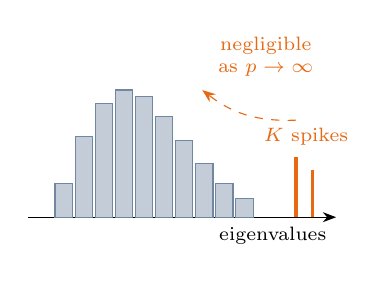
\begin{tikzpicture}[scale=0.85, every node/.style={font=\scriptsize}]
      \draw[-{Stealth}] (0,0) -- (4.6,0) node[below left] {eigenvalues};
      % MP bulk
      \foreach \x/\h in {0.4/0.5,0.7/1.2,1.0/1.7,1.3/1.9,1.6/1.8,1.9/1.5,2.2/1.15,2.5/0.8,2.8/0.5,3.1/0.28}{
        \draw[fill=navy!25, draw=navy!60] (\x,0) rectangle (\x+0.26,\h);
      }
      % spikes
      \draw[very thick, ensorange] (4.0,0) -- (4.0,0.9);
      \draw[very thick, ensorange] (4.25,0) -- (4.25,0.7);
      \node[ensorange] at (4.15,1.2) {$K$ spikes};
      \node[ensorange, align=center] at (3.55,2.4) {negligible\\ as $p\to\infty$};
      \draw[-{Stealth}, ensorange, dashed] (4.0,1.45) to[bend left=20] (2.6,1.9);
    \end{tikzpicture}
    \end{center}
  \end{columns}
  \takeaway{In the proportional regime, a finite number of shifted directions does not affect the limiting prediction risk.}
\end{frame}

% ---------- 13 ----------
\begin{frame}{Optimally tuned ridge: pooling dominates (Thm 2.4, Cor 2.6)}
  Random effects, $K=2$, $\Sigma = \mathbb{I}$, both methods optimally tuned and weighted:
  \[
    \frac{R^\star_{\mathrm{ens}} - \sigma_\star^2}{R^\star_{\mathrm{pool}} - \sigma_\star^2}
    \;=\; \frac{\kappa_1\kappa_2\,(1-\kappa_1\kappa_2)}{\kappa_0\,(\kappa_1+\kappa_2-2\kappa_1\kappa_2)} \;+\; o_{\mathbb{P}}(1)
    \;\;\textcolor{wingreen}{\bm{>}\; 1}
  \]
  where $\kappa_\ell = \kappa(\gamma_\ell)$ solves an explicit quadratic in the aspect ratio and the signal-to-noise ratio.
  \vspace{2mm}
  \begin{itemize}
    \item The inequality holds regardless of the angles, norms, or covariance structure of the cluster means
    \item The excess-risk ratio is strictly greater than one, not merely bounded below by one
  \end{itemize}
\end{frame}

% ---------- 14 ----------
\begin{frame}{Intuition for the ridge result}
  \begin{itemize}
    \item Because $\bbeta$ is shared, samples from every cluster are equally informative about the target; splitting reduces the effective sample size of each fit without any compensating reduction in bias
    \item Each base learner operates at aspect ratio $K\gamma_0$ and therefore has higher variance; averaging $K$ learners trained on disjoint data recovers only part of the difference
    \item The variance reduction achieved by averaging can also be achieved --- more efficiently --- by increasing the ridge penalty
  \end{itemize}
  \vspace{2mm}
  {\small\textcolor{softgray}{Consistent with Patil et al.\ (2023): subsampling ensembles act as implicit ridge regularization, and explicit tuning weakly dominates.}}
\end{frame}

% ---------- 15 ----------
\begin{frame}{Ridgeless regression: regime-dependent behavior (Cor 2.6)}
  $K=2$, $n_1 = n_2$, $\gamma = p/n$:
  \begin{columns}[T]
    \column{0.5\textwidth}
    \vspace{1mm}
    \begin{center}
    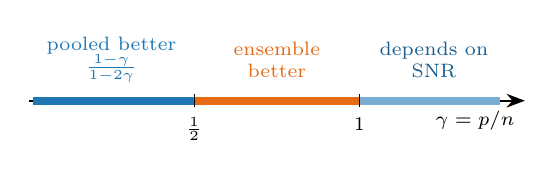
\begin{tikzpicture}[scale=1.05, every node/.style={font=\scriptsize}]
      \draw[-{Stealth}, thick] (0,0) -- (6.0,0) node[below left] {$\gamma = p/n$};
      \draw[line width=3pt, poolblue] (0.05,0) -- (2.0,0);
      \draw[line width=3pt, ensorange] (2.0,0) -- (4.0,0);
      \draw[line width=3pt, poolblue!60] (4.0,0) -- (5.7,0);
      \foreach \x/\l in {2.0/{\tfrac12}, 4.0/{1}}{\draw (\x,-0.08) -- (\x,0.08) node[below=5pt, black] {$\l$};}
      \node[poolblue, align=center] at (1.0,0.5) {pooled better\\ $\frac{1-\gamma}{1-2\gamma}$};
      \node[ensorange, align=center] at (3.0,0.5) {ensemble\\ better};
      \node[poolblue!80!black, align=center] at (4.9,0.5) {depends on\\ SNR};
    \end{tikzpicture}
    \end{center}
    \vspace{1mm}
    {\small For $\gamma > 1$, the pooled learner is better iff
    $\dfrac{\sigma_\varepsilon^2}{\tau^2} < \dfrac{(2\gamma+1)(2\gamma-1)(\gamma-1)}{4\gamma^2(3\gamma-1)}$}
    \column{0.46\textwidth}
    \begin{center}
      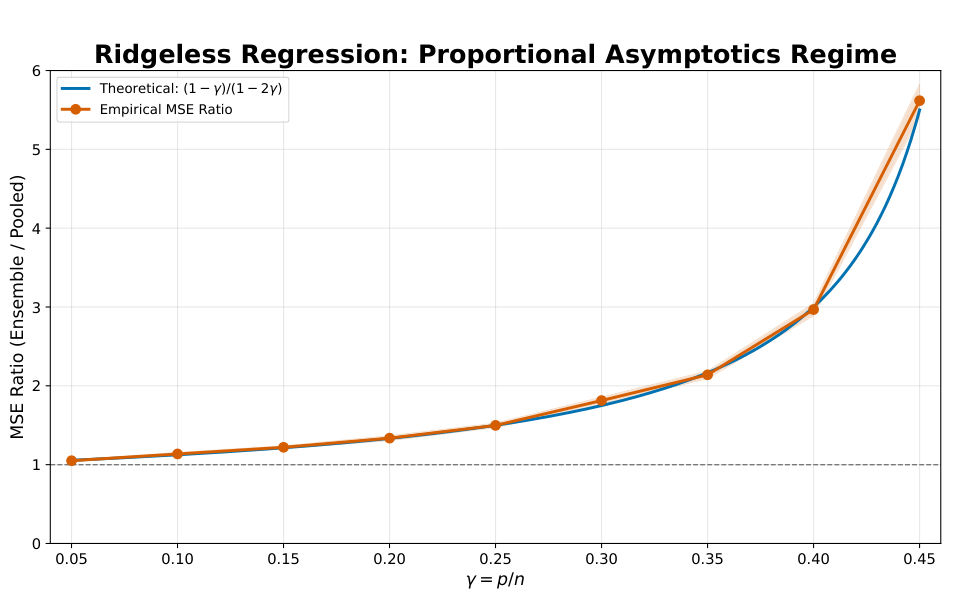
\includegraphics[width=\textwidth]{figs/fig1.png}\\
      {\scriptsize Simulated ratio matches the limit $\tfrac{1-\gamma}{1-2\gamma}$ for $\gamma < \tfrac12$ (Figure 1)}
    \end{center}
  \end{columns}
  \takeaway{Without regularization, the comparison is determined by $p/n$ relative to the two interpolation thresholds.}
\end{frame}

% ---------- 16 ----------
\begin{frame}{Intuition for the ridgeless regimes}
  \textbf{Why the ensemble is better for $\tfrac{n}{2} < p < n$:}
  \begin{itemize}
    \item In this range each base learner is past its interpolation threshold ($p/n_\ell > 1$), where overparameterization acts as implicit regularization and stabilizes the variance
    \item The pooled learner, by contrast, is approaching its own threshold at $p \approx n$, where its variance diverges
    \item The ensemble's risk peak at $p \approx n/2$ is roughly a quarter the size of the pooled peak, since it averages two predictors trained on disjoint samples
  \end{itemize}
  \vspace{1mm}
  \textbf{The role of noise for $\gamma > 1$:}
  \begin{itemize}
    \item Implicit regularization primarily suppresses variance from label noise, so the ensemble is favored at low SNR and the pooled learner at high SNR
  \end{itemize}
\end{frame}

% ---------- 17 ----------
\begin{frame}{Relation to Patil et al.\ (2023)}
  \begin{center}
  \renewcommand{\arraystretch}{1.3}
  \begin{tabular}{lcc}
     & \textcolor{softgray}{Patil et al.\ (2023)} & \textbf{This paper}\\
    \hline
    Data & i.i.d. & covariate shift, $K$ clusters\\
    Partition & uniformly random & along the true cluster structure\\
    Conclusion & tuned ridge optimal & tuned ridge optimal\\
  \end{tabular}
  \end{center}
  \vspace{3mm}
  \begin{itemize}
    \item The conclusions of the i.i.d.\ analysis persist under covariate heterogeneity and heterogeneity-aware partitioning
    \item In particular, partitioning along the true cluster structure provides no advantage over random splitting (Section 4)
  \end{itemize}
\end{frame}

% ---------- 18 ----------
\begin{frame}{Proof overview}
  \begin{center}
  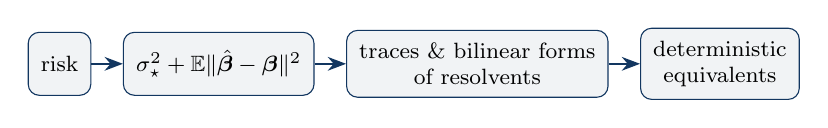
\begin{tikzpicture}[node distance=3mm and 4mm, every node/.style={font=\footnotesize}]
    \tikzset{pbox/.style={draw=navy, rounded corners, fill=navy!6, minimum height=8mm, inner sep=1.6mm, align=center}}
    \node[pbox] (a) {risk};
    \node[pbox, right=of a] (b) {$\sigma_\star^2 + \E\|\hat\bbeta - \bbeta\|^2$};
    \node[pbox, right=of b] (c) {traces \& bilinear forms\\ of resolvents};
    \node[pbox, right=of c] (d) {deterministic\\ equivalents};
    \draw[-{Stealth}, thick, navy] (a) -- (b);
    \draw[-{Stealth}, thick, navy] (b) -- (c);
    \draw[-{Stealth}, thick, navy] (c) -- (d);
  \end{tikzpicture}
  \end{center}
  \vspace{2mm}
  \begin{itemize}
    \item The overall structure follows standard random matrix theory arguments (Marchenko--Pastur; anisotropic local laws, Knowles--Yin 2017)
    \item Two complications relative to the i.i.d.\ setting: non-zero cluster means make the sample covariances non-centered, and the ensemble risk couples resolvents of different clusters
  \end{itemize}
  \vspace{1mm}
  The next five slides describe the main techniques used to handle these.
\end{frame}

% ---------- 19 ----------
\begin{frame}{Mean shifts as finite-rank perturbations}
  Decompose the pooled design matrix: \quad $\X_{\mathrm{pool}} = \mathbb{Z}_0\Sigma^{1/2} + M$, \qquad $\operatorname{rank}(M) \le K$
  \[
    \operatorname{rank}\big(\widehat\Sigma_{\mathrm{pool}} - \widehat\Sigma^{\,0}_{\mathrm{pool}}\big) \;\le\; 3K,
    \qquad\quad
    \Big|\tfrac1p\Tr f(A) - \tfrac1p\Tr f(B)\Big| \;\lesssim\; \frac{\operatorname{rank}(A-B)}{p} \;\to\; 0
  \]
  \vspace{1mm}
  \begin{itemize}
    \item Normalized trace functionals are insensitive to a rank-$3K$ change
    \item Consequently, for all spectral quantities (variance terms, random-effects bias), the means can be removed without affecting the limit
  \end{itemize}
\end{frame}

% ---------- 20 ----------
\begin{frame}{Fixed effects: where the means enter}
  Under fixed effects the bias involves the \textbf{bilinear form} $\bbeta^\top G_{\mathrm{pool}}\,\bbeta$ rather than a normalized trace, so it can concentrate on the $K$ mean directions.
  \vspace{1mm}

  Applying Woodbury's identity separates the mean directions from the centered part:
  \[
    \mathcal{K}_{\gamma,\bmu}(\rho) \;=\; Q_\gamma(\rho)\;-\;
    \frac{Q_\gamma(\rho)\,\bmu\bmu^\top Q_\gamma(\rho)}{1 + \gamma s_\gamma(\rho) + \bmu^\top Q_\gamma(\rho)\bmu}
  \]
  \begin{itemize}
    \item This is the $\mathcal{K}$ functional appearing in the fixed-effects theorems
    \item It quantifies the component of $\bbeta$ lying along the mean directions
  \end{itemize}
  \takeaway{Mean shifts do not affect spectral functionals, but they do enter bilinear forms in $\bbeta$; the effect is a $K \times K$ correction.}
\end{frame}

% ---------- 21 ----------
\begin{frame}{Leave-one-out arguments for the cross terms}
  The most delicate terms are bilinear forms in which the resolvent depends on the rows appearing in the form (cross-cluster products, mean directions).
  \begin{itemize}
    \item Sherman--Morrison updates remove the relevant row from the resolvent, restoring independence at the cost of an explicit rank-one correction of order $1/n$
    \item Bounding the second moment of the off-diagonal sums requires leaving out up to four rows and classifying index quadruples by their overlap:
    \[
      \E U_m^2 \;\lesssim\; \underbrace{m^2 p}_{\text{same pair}} + \underbrace{m^3\,\tfrac{p}{n}}_{\text{one shared index}} + \underbrace{m^4\,\tfrac{p}{n^2}}_{\text{all distinct}}
      \;\;\Rightarrow\;\; \tfrac{1}{m^2}U_m = o_{\mathbb{P}}(1)
    \]
    \item Each removed dependency contributes a factor of $1/n$, which makes the combinatorial count converge
  \end{itemize}
\end{frame}

% ---------- 22 ----------
\begin{frame}{Ridgeless results as limits of ridge results}
  The ridgeless case does not require a separate analysis:
  \begin{itemize}
    \item With high probability, all nonzero eigenvalues of $\widehat\Sigma_{\mathrm{pool}}$ lie in a fixed interval $[c, 1/c]$
    \item On this event, pseudoinverse quantities are uniform limits of the corresponding ridge quantities as $\rho \downarrow 0$
    \item The under- and overparameterized regimes are handled through the rank of the projection: $\tfrac1p\Tr(\mathbb{I} - P_{\mathcal{C}(\X)}) \to 1 - \tfrac{1}{\gamma_0}$
  \end{itemize}
  \vspace{2mm}
  \[
    B_+ = \lim_{\rho_0 \downarrow 0} \rho_0^2\,[-\psi_0'(\rho_0)],
    \qquad
    V_+ = \lim_{\rho_0 \downarrow 0} V_{\gamma_0}(\rho_0)
  \]
\end{frame}

% ---------- 23 ----------
\begin{frame}{Proof of Corollary 2.6: strict inequality}
  Substituting $h(u) = \tfrac{\alpha}{u} - u - \alpha + 1$ (strictly decreasing on $(0,1)$) into the fixed-point equation for $\kappa$ gives
  \[
    h(\kappa(\gamma)) = \tfrac{1}{\gamma},
    \qquad
    \underbrace{\tfrac{1}{\gamma_0} = \tfrac{1}{\gamma_1} + \tfrac{1}{\gamma_2}}_{\text{sample sizes add}}
    \;\;\Longrightarrow\;\;
    \boxed{h(\kappa_0) = h(\kappa_1) + h(\kappa_2)}
  \]
  \begin{columns}[T]
    \column{0.6\textwidth}
    \begin{itemize}
      \item Under pooling, the risk parameter composes additively through $h$ --- analogous to parallel composition
      \item A direct algebraic computation shows the ensemble's combined risk $q(\kappa_1,\kappa_2)$ satisfies $h(q) < h(\kappa_1) + h(\kappa_2)$
      \item Since $h$ is decreasing, this gives $q > \kappa_0$: the ensemble's excess risk is strictly larger
    \end{itemize}
    \column{0.36\textwidth}
    \begin{center}
    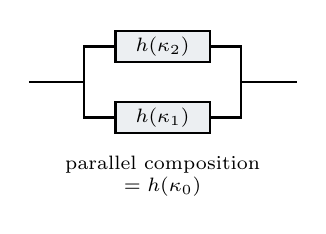
\begin{tikzpicture}[every node/.style={font=\scriptsize}]
      \draw[thick] (-0.4,0.7) -- (0.3,0.7);
      \draw[thick] (0.3,0.7) -- (0.3,1.15) -- (0.7,1.15);
      \draw[thick] (0.3,0.7) -- (0.3,0.25) -- (0.7,0.25);
      \draw[thick, fill=navy!8] (0.7,0.95) rectangle (1.9,1.35);
      \node at (1.3,1.15) {$h(\kappa_2)$};
      \draw[thick, fill=navy!8] (0.7,0.05) rectangle (1.9,0.45);
      \node at (1.3,0.25) {$h(\kappa_1)$};
      \draw[thick] (1.9,1.15) -- (2.3,1.15) -- (2.3,0.7);
      \draw[thick] (1.9,0.25) -- (2.3,0.25) -- (2.3,0.7);
      \draw[thick] (2.3,0.7) -- (3.0,0.7);
      \node[align=center] at (1.3,-0.5) {parallel composition\\ $= h(\kappa_0)$};
    \end{tikzpicture}
    \end{center}
  \end{columns}
\end{frame}

% ---------- 24 ----------
\begin{frame}{Simulation design}
  \begin{itemize}
    \item $n = 2000$, $K = 2$ Gaussian clusters; $p$ ranges from $250$ to $6000$, spanning both interpolation thresholds ($p = 1000$ and $p = 2000$)
    \item Cluster-mean geometry is varied to test the prediction that it has no effect: angle between $\bmu_1, \bmu_2 \in \{30^\circ, 60^\circ, 90^\circ\}$, $\|\bmu_2\| \in \{1, 5, 10\}$
    \item Ridge penalty tuned by leave-one-out cross-validation separately for every learner; ridgeless solutions computed via SVD; 100 repetitions with 95\% confidence intervals
  \end{itemize}
\end{frame}

% ---------- 25 ----------
\begin{frame}{Simulation results: ridge}
  \begin{columns}[T]
    \column{0.48\textwidth}
    \centering 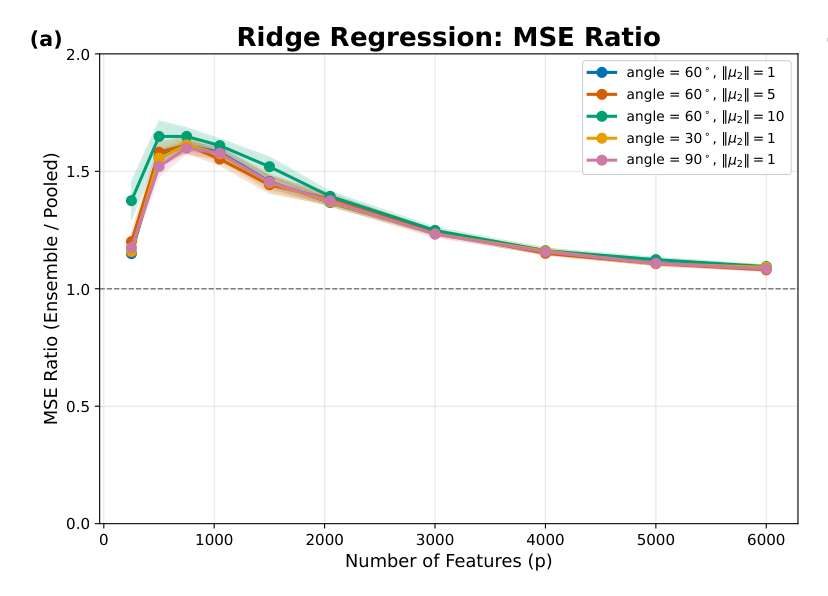
\includegraphics[width=\textwidth]{figs/fig2a.png}
    \column{0.48\textwidth}
    \centering 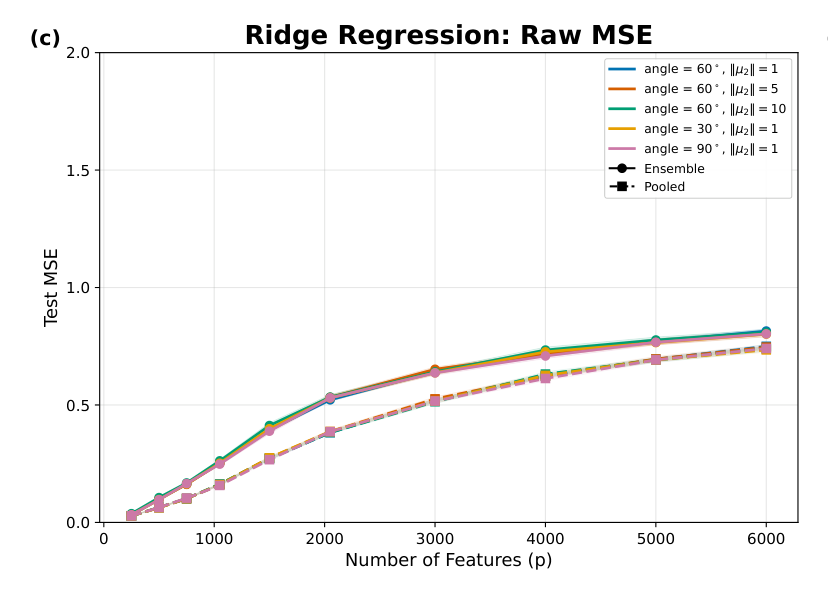
\includegraphics[width=\textwidth]{figs/fig2c.png}
  \end{columns}
  \vspace{1mm}
  \begin{itemize}
    \item The pooled learner is better at every value of $p$: the MSE ratio ranges from $1.06$ to $1.62$, and the raw MSE curves are smooth and monotone, with no interpolation peaks
    \item The curves for the different geometry configurations are indistinguishable
  \end{itemize}
\end{frame}

% ---------- 26 ----------
\begin{frame}{Simulation results: ridgeless}
  \begin{columns}[T]
    \column{0.48\textwidth}
    \centering 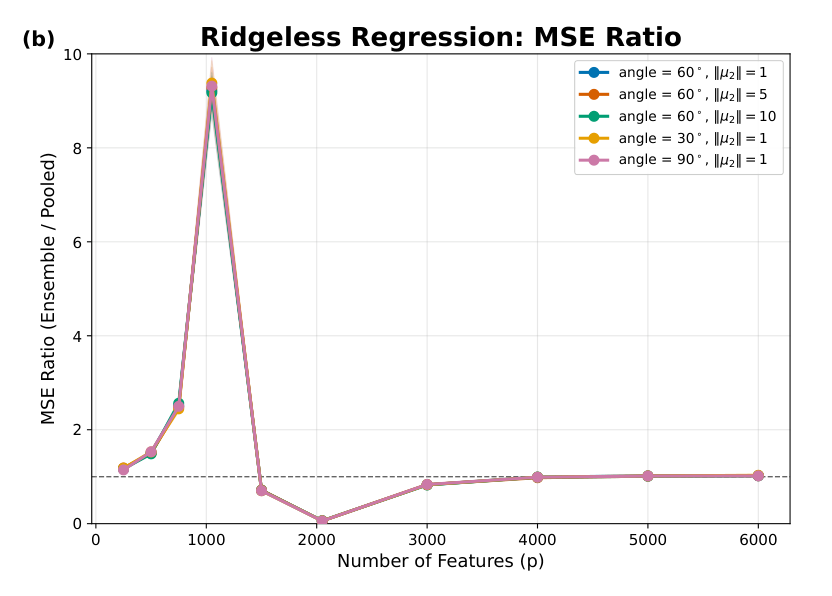
\includegraphics[width=\textwidth]{figs/fig2b.png}
    \column{0.48\textwidth}
    \centering 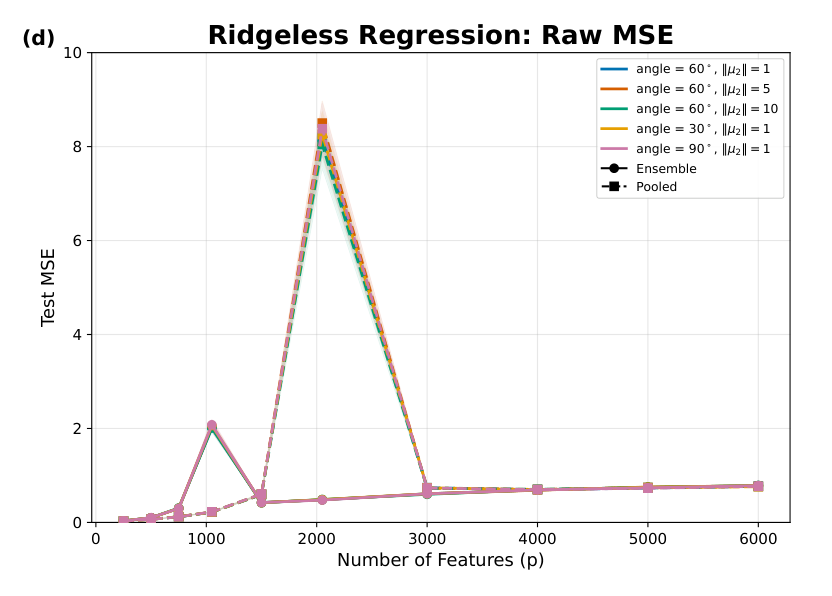
\includegraphics[width=\textwidth]{figs/fig2d.png}
  \end{columns}
  \vspace{1mm}
  \begin{itemize}
    \item The ensemble's risk peaks at $p \approx n_1$ (ratio near $10$); the ratio drops below $1$ in the intermediate regime $n_1 < p < n$; the pooled peak at $p \approx n$ is roughly four times larger; both methods converge to the null risk for large $p$
  \end{itemize}
\end{frame}

% ---------- 27 ----------
\begin{frame}{Ablations: cluster geometry and partition structure}
  \begin{itemize}
    \item Varying the angle and norms of the cluster means has no detectable effect: the curves lie within each other's confidence intervals at almost every $p$
    \item Splitting the data randomly, rather than along the true clusters, produces identical results
    \item So does the fully i.i.d.\ setting with a two-way random split
  \end{itemize}
  \vspace{2mm}
  The relevant feature of the partition is not its alignment with the cluster structure, but simply that it divides the sample in half --- i.e., that it changes the aspect ratio from $\gamma$ to $2\gamma$.
\end{frame}

% ---------- 28 ----------
\begin{frame}{Practical implications}
  \begin{itemize}
    \item When heterogeneity is confined to the covariates and the conditional model is shared, pooling with a tuned ridge penalty is preferable to cluster-wise ensembling
    \item An observed ensemble advantage in applications therefore points to concept shift, model misspecification, or nonlinearity rather than to covariate heterogeneity itself
    \item Combined with Ramchandran \& Mukherjee (2021), this suggests the random-forest gains under covariate shift stem from properties of the learner (nonlinearity, local adaptivity) rather than from the shift
    \item Unregularized pooled fits should be avoided near $p \approx n$
  \end{itemize}
\end{frame}

% ---------- 29 ----------
\begin{frame}{Limitations and future work}
  \begin{itemize}
    \item The analysis covers mean shifts only; joint shifts in mean and covariance appear reachable with the same arguments
    \item Cluster labels are assumed known; estimated memberships introduce additional uncertainty
    \item The linear model is well-specified; nonlinear extensions could follow the template of Hastie et al.\ (2019)
    \item Under fixed effects, the optimal weights depend on quantities that are difficult to estimate in the proportional regime; adaptive selection between pooling and ensembling remains open
    \item Behavior at the interpolation thresholds under covariate shift is not analyzed
  \end{itemize}
\end{frame}

% ---------- 30 ----------
\begin{frame}{Summary}
  \begin{enumerate}
    \item For every optimally tuned ridge penalty $\lambda > 0$, the pooled learner outperforms the optimally weighted ensemble under pure covariate shift
    \item For ridgeless regression, the comparison is governed by $p/n$ relative to the two interpolation thresholds; the ensemble is preferable only where splitting acts as implicit regularization
    \item The geometry of the cluster means --- and the alignment of the partition with the true clusters --- has no effect on the asymptotic comparison
  \end{enumerate}
  \vspace{4mm}
  \begin{center}
    \colorbox{navy!10}{\parbox{0.85\textwidth}{\centering\textcolor{navy}{Under pure covariate shift, the benefit of cluster-wise ensembling for linear methods reduces to implicit regularization --- which explicit tuning dominates.}}}
  \end{center}
  \vspace{2mm}
  \centering Thank you.
\end{frame}

% ---------- backup ----------
\begin{frame}[plain]
  \centering\Huge\textcolor{navy}{Backup}
\end{frame}

\begin{frame}{Backup: ensemble risk, random effects (Theorem 2.3)}
  \small
  With $\E(\bbeta) = 0$, $\mathrm{Var}(\bbeta) = \tfrac{\tau^2}{p}\mathbb{I}$:
  \begin{align*}
    R_{\mathrm{ens},\bm\rho}(\bm w)
    &= \sigma_\star^2
    + \sum_{\ell=1}^{K} w_\ell^2 \Big\{ \tau^2 \rho_\ell^2\,[-a'_{\gamma_\ell}(\rho_\ell)] + \sigma_\varepsilon^2 V_{\gamma_\ell}(\rho_\ell) \Big\}\\
    &\qquad + 2\tau^2 \!\!\sum_{1 \le \ell < j \le K}\!\! w_\ell w_j\, \rho_\ell \rho_j\, \tfrac1p \Tr(Q_\ell Q_j) + o(1)
  \end{align*}
  Ridgeless: $\rho_\ell \downarrow 0$ limits. Fixed effects: replace $\tau^2\rho_\ell^2[-a']$ by $\rho_\ell^2[-\psi'_\ell]$ and cross terms by $\bbeta^\top \mathcal{K}_\ell \mathcal{K}_j \bbeta$.
\end{frame}

\begin{frame}{Backup: pooled risk (Theorem 2.5)}
  \small
  Random effects:
  \[
    R_{\mathrm{pool},\rho_0} = \sigma_\star^2 + \tau^2\rho_0^2\,[-a'_{\gamma_0}(\rho_0)] + \sigma_\varepsilon^2 V_{\gamma_0}(\rho_0) + o(1)
  \]
  Fixed effects, with $U_0 = [\sqrt{\pi_1}\bmu_1, \ldots, \sqrt{\pi_K}\bmu_K]$ and $\psi_0(\rho) = \bbeta^\top \mathcal{K}_{\gamma_0, U_0}(\rho)\,\bbeta$:
  \[
    R_{\mathrm{pool},\rho_0} = \sigma_\star^2 + \rho_0^2\,[-\psi_0'(\rho_0)] + \sigma_\varepsilon^2 V_{\gamma_0}(\rho_0) + o(1)
  \]
  Ridgeless: $\rho_0 \downarrow 0$ limits of both.
\end{frame}

\begin{frame}{Backup: the $\kappa$ fixed point (Corollary 2.6)}
  \small
  With $\alpha = \sigma_\varepsilon^2 / \tau^2$ and $\rho^\star_\ell = \gamma_\ell\alpha$ the optimal tuning:
  \[
    \kappa(\gamma) = \frac{-(\alpha - 1 + \gamma^{-1}) + \sqrt{(\alpha - 1 + \gamma^{-1})^2 + 4\alpha}}{2},
    \qquad
    \kappa^2 + \Big(\alpha - 1 + \tfrac{1}{\gamma}\Big)\kappa - \alpha = 0
  \]
  $0 < \kappa(\gamma) < 1$ always; the pooled learner is no worse than \emph{any} convex ensemble iff
  $\kappa_0 \le \min_{\bm w} \bm w^\top B \bm w$ with
  $B = \operatorname{diag}(\kappa_1(1-\kappa_1), \ldots) + \bm\kappa\bm\kappa^\top$.
\end{frame}

\end{document}
